% \documentclass{standalone}
% \usepackage{tikz}
% \usepackage{tikz-3dplot}

% \begin{document}

% \tdplotsetmaincoords{70}{80} % Set the viewing angle

% \begin{tikzpicture}[scale=1.4, tdplot_main_coords]

% \node[anchor=north] at (0, 1.3, 7.3) {\Huge LP in the standard (equality) form};

% % Define vertices
% \coordinate (A) at (5,0,0);
% \coordinate (B) at (0,5,0);
% \coordinate (C) at (0,0,5);
% \coordinate (D) at (0,0,0);

% % Draw simplex edges
% \draw[thick] (A) -- (B) -- (C) -- cycle;

% % Fill simplex
% \filldraw[fill=gray!40, fill opacity=0.3] (A) -- (B) -- (C) -- cycle;

% % Draw axes
% \draw[-latex, gray] (-10,0,0) -- (10,0,0) node[anchor=north east]{\Huge{$x_1$}};
% \draw[-latex, gray] (0,-4,0) -- (0,6,0) node[anchor=north west]{\Huge{$x_2$}};
% \draw[-latex, gray] (0,0,-4) -- (0,0,6) node[anchor=south]{\Huge{$x_3$}};

% % Add equation text
% \node[anchor=north] at (2,1.85,2) {\Huge{$\tilde{\mathbf{A}}\tilde{\mathbf{x}} = \mathbf{b}$}};
% \node[anchor=north] at (0, -0.3, -0.1) {\Huge{$\mathbf{0}$}};

% % Draw dots at the points where the simplex crosses the axes
% \coordinate (Ax) at (5,0,0);
% \coordinate (By) at (0,5,0);
% \coordinate (Cz) at (0,0,5);
% \filldraw [black] (Ax) circle (1pt);
% \filldraw [black] (By) circle (1pt);
% \filldraw [black] (Cz) circle (1pt);

% \end{tikzpicture}

% \end{document}

\documentclass{standalone}
\usepackage{tikz}

\begin{document}
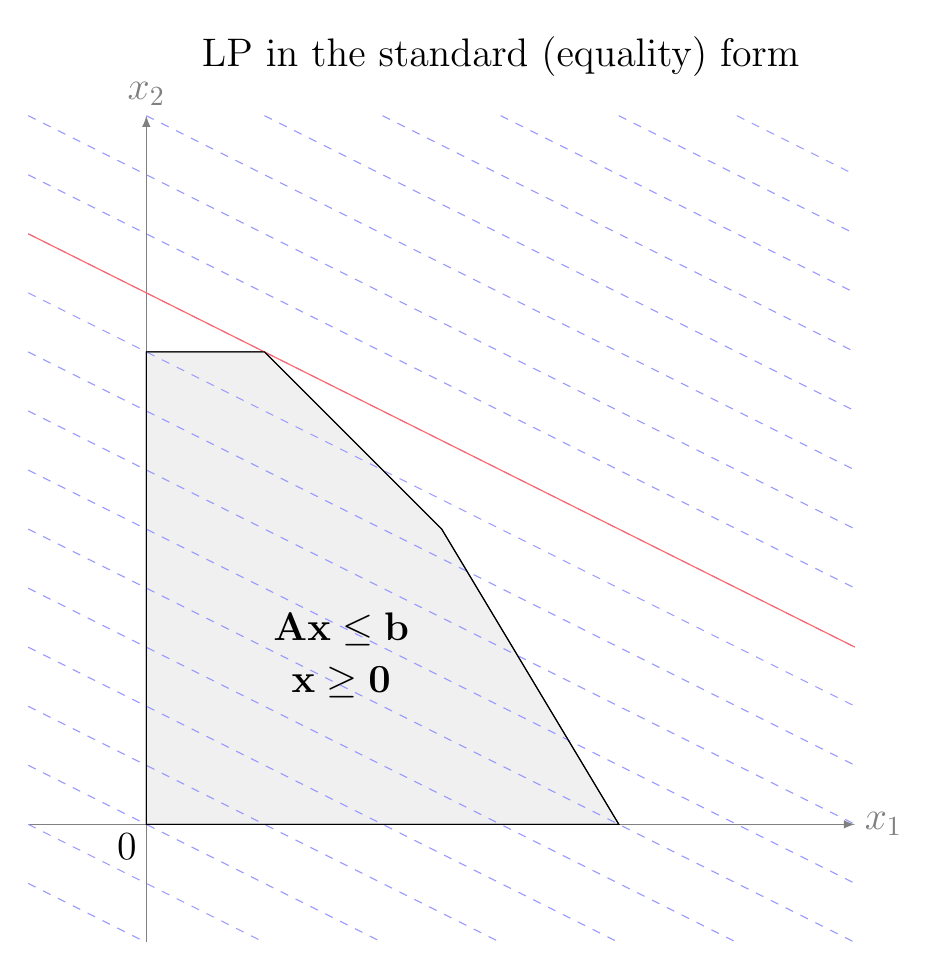
\begin{tikzpicture}[scale=1.5]
    \node[anchor=north] at (3,6.75) {\Large{LP in the standard (equality) form}};

    % Define vertices
    \coordinate (O) at (0,0);
    \coordinate (A) at (0,4);
    \coordinate (B) at (1,4);
    \coordinate (C) at (2.5,2.5);
    \coordinate (D) at (4,0);

    % Draw axes
    \draw[-latex, gray] (-1,0) -- (6,0) node[right] {\Large{$x_1$}};
    \draw[-latex, gray] (0,-1) -- (0,6) node[above] {\Large{$x_2$}};
    
    % Draw axes
    \draw[solid, black] (O) -- (A) -- (B) -- (C) -- (D) -- cycle;
    
    % Draw the region defined by the constraint
    \fill[gray!40, fill opacity=0.3] (O) -- (A) -- (B) -- (C) -- (D) -- cycle;
    
    % Add labels
    \node at (1.65, 1.65) {\Large{$\mathbf{A}\mathbf{x} \leq \mathbf{b}$}};
    \node at (1.65, 1.2) {\Large{$\mathbf{x} \geq \mathbf{0}$}};
    \node[below left] at (0,0) {\Large $0$};

    % Draw contours of x1 + 2*x2
    \foreach \c in {-2,-1,0,1,2,3,4}{
        \draw[dashed,blue!40] (-1, {(\c + 1)/2}) -- ({\c + 2},-1);
    }
    \foreach \c in {5,6,7,8,9,10}{
        \draw[dashed,blue!40] (-1, {(\c + 1)/2}) -- (6,{(\c - 6)/2});
    }
    \foreach \c in {11,12,13,14,15,16,17}{
        \draw[dashed,blue!40] ({\c - 12}, 6) -- (6,{(\c - 6)/2});
    }
    \draw[solid,red!60!] (-1, 5) -- (6,1.5);

    % Boundary outline
    \draw[solid,black] (O) -- (A) -- (B) -- (C) -- (D) -- cycle;

\end{tikzpicture}
\end{document}
